\documentclass{article}

% if you need to pass options to natbib, use, e.g.:
\PassOptionsToPackage{sort&compress,numbers}{natbib}
% before loading nips_2017
%
% to avoid loading the natbib package, add option nonatbib:
% \usepackage[nonatbib]{nips_2017}

% \usepackage{nips_2017}
% \usepackage[final]{nips_2017}

% to compile a camera-ready version, add the [final] option, e.g.:
\usepackage[final]{nips_2017}

\usepackage[utf8]{inputenc} % allow utf-8 input
\usepackage[T1]{fontenc}    % use 8-bit T1 fonts
\usepackage{hyperref}       % hyperlinks
\usepackage{url}            % simple URL typesetting
\usepackage{booktabs}       % professional-quality tables
\usepackage{amsfonts}       % blackboard math symbols
\usepackage{nicefrac}       % compact symbols for 1/2, etc.
\usepackage{microtype}      % microtypography
\usepackage[pdftex]{graphicx}
\usepackage{dsfont}
\usepackage{subcaption}
\usepackage{amsmath}
\usepackage{amssymb}
\usepackage{xspace}
\usepackage{enumitem}

% \usepackage[sort]{cite}

% additional definitions
\usepackage{color}
\definecolor{darkred}{RGB}{180,50,20}
\definecolor{darkgreen}{RGB}{20,180,50}
\definecolor{purple}{RGB}{90,20,90}
\definecolor{fr}{RGB}{60,125,161}
\newcommand{\ow}[1] {\emph{\textcolor{darkred}{OW: #1}}}
\newcommand{\es}[1] {\emph{\textcolor{darkgreen}{ES: #1}}}
\newcommand{\td}[1] {\emph{\textcolor{purple}{TD: #1}}}
\newcommand{\deepak}[1] {\emph{\textcolor{darkred}{DP: #1}}}
\newcommand{\rz}[1] {\emph{\textcolor{fr}{rz: #1}}}
%\setlength\abovedisplayskip{10pt}


\newcommand{\pp}{\texttt{pix2pix}\xspace}
\newcommand{\ppn}{\texttt{pix2pix+noise}\xspace}
\newcommand{\cinfogan}{\texttt{cLR-GAN}\xspace}
\newcommand{\cae}{\texttt{cAE-GAN}\xspace}
\newcommand{\cvaegan}{\texttt{cVAE-GAN}\xspace}
\newcommand{\cvaeganp}{\texttt{cVAE-GAN++}\xspace}
\newcommand{\bicycle}{\texttt{BicycleGAN}\xspace} %cVAE-LR-GAN
\newcommand{\G}{G\xspace}
\newcommand{\D}{D\xspace}
\newcommand{\E}{E\xspace}
\newcommand{\A}{\mathbf{A}\xspace}
\newcommand{\B}{\mathbf{B}\xspace}
\newcommand{\Bh}{\widehat{\mathbf{B}}\xspace}
\newcommand{\z}{\mathbf{z}\xspace}
\newcommand{\zh}{\widehat{\mathbf{z}}\xspace}
% \newcommand{\L}{\mathcal{L}\xspace}
\newif\ifsubmit
\submitfalse

\ifsubmit
\newcommand{\jy}[1]{}
\newcommand{\revjy}[1]{}
\else
\newcommand{\jy}[1]{\textcolor{blue}{JY: #1}}
\newcommand{\revjy}[1]{\textcolor{blue}{#1}}
\fi


% Papers may be only up to 8 pages long, including figures. An additional ninth page containing only cited references and acknowledgments is allowed. Papers that exceed 9 pages will be rejected without review.

% \usepackage{fancyhdr}
% \usepackage{pdfpages}
% \pagestyle{fancy}
% \fancyhf{}
% \fancyhead[C]{\textbf{DRAFT - Please do not distribute}}
% \fancyfoot[C]{\thepage}


\title{Toward Multimodal Image-to-Image Translation}


% The \author macro works with any number of authors. There are two
% commands used to separate the names and addresses of multiple
% authors: \And and \AND.
%
% Using \And between authors leaves it to LaTeX to determine where to
% break the lines. Using \AND forces a line break at that point. So,
% if LaTeX puts 3 of 4 authors names on the first line, and the last
% on the second line, try using \AND instead of \And before the third
% author name.


\author{
  Jun-Yan Zhu\\
  UC Berkeley\\
%   \texttt{\{junyanz,rich.zhang,pathak\}@eecs.berkeley.edu} \\
  \And
  Richard Zhang\\
  UC Berkeley\\
  \And
  Deepak Pathak\\
  UC Berkeley\\
  \AND
  Trevor Darrell\\
  UC Berkeley\\
  \And
    Alexei A. Efros\\
    UC Berkeley\\
%   \texttt{\{trevor,efros\}@eecs.berkeley.edu} \\
  \And
  Oliver Wang\\
  Adobe Research\\
  \And
  Eli Shechtman\\
  Adobe Research\\
%   \texttt{\{elishe,owang\}@adobe.com} \\
}


\begin{document}
% \nipsfinalcopy is no longer used

\maketitle

\begin{abstract}
Diffusion Models have emerged as powerful generative models for high-quality image synthesis, with many subsequent image editing techniques based on them. However, the ease of text-based image editing introduces significant risks, such as malicious editing for scams or intellectual property infringement. Previous works have attempted to safeguard images from diffusion-based editing by adding imperceptible perturbations. These methods are costly and specifically target prevalent Latent Diffusion Models (LDMs), while Pixel-domain Diffusion Models (PDMs) remain largely unexplored and robust against such attacks. Our work addresses this gap by proposing a novel attacking framework with a feature representation attack loss that exploits vulnerabilities in denoising UNets and a latent optimization strategy to enhance the naturalness of protected images. Extensive experiments demonstrate the effectiveness of our approach in attacking dominant PDM-based editing methods (e.g., SDEdit) while maintaining reasonable protection fidelity and robustness against common defense methods. Additionally, our framework is extensible to LDMs, achieving comparable performance to existing approaches.
\end{abstract}


\section{Introduction}
\label{sec:intro}

\begin{figure*}[t]
\centering
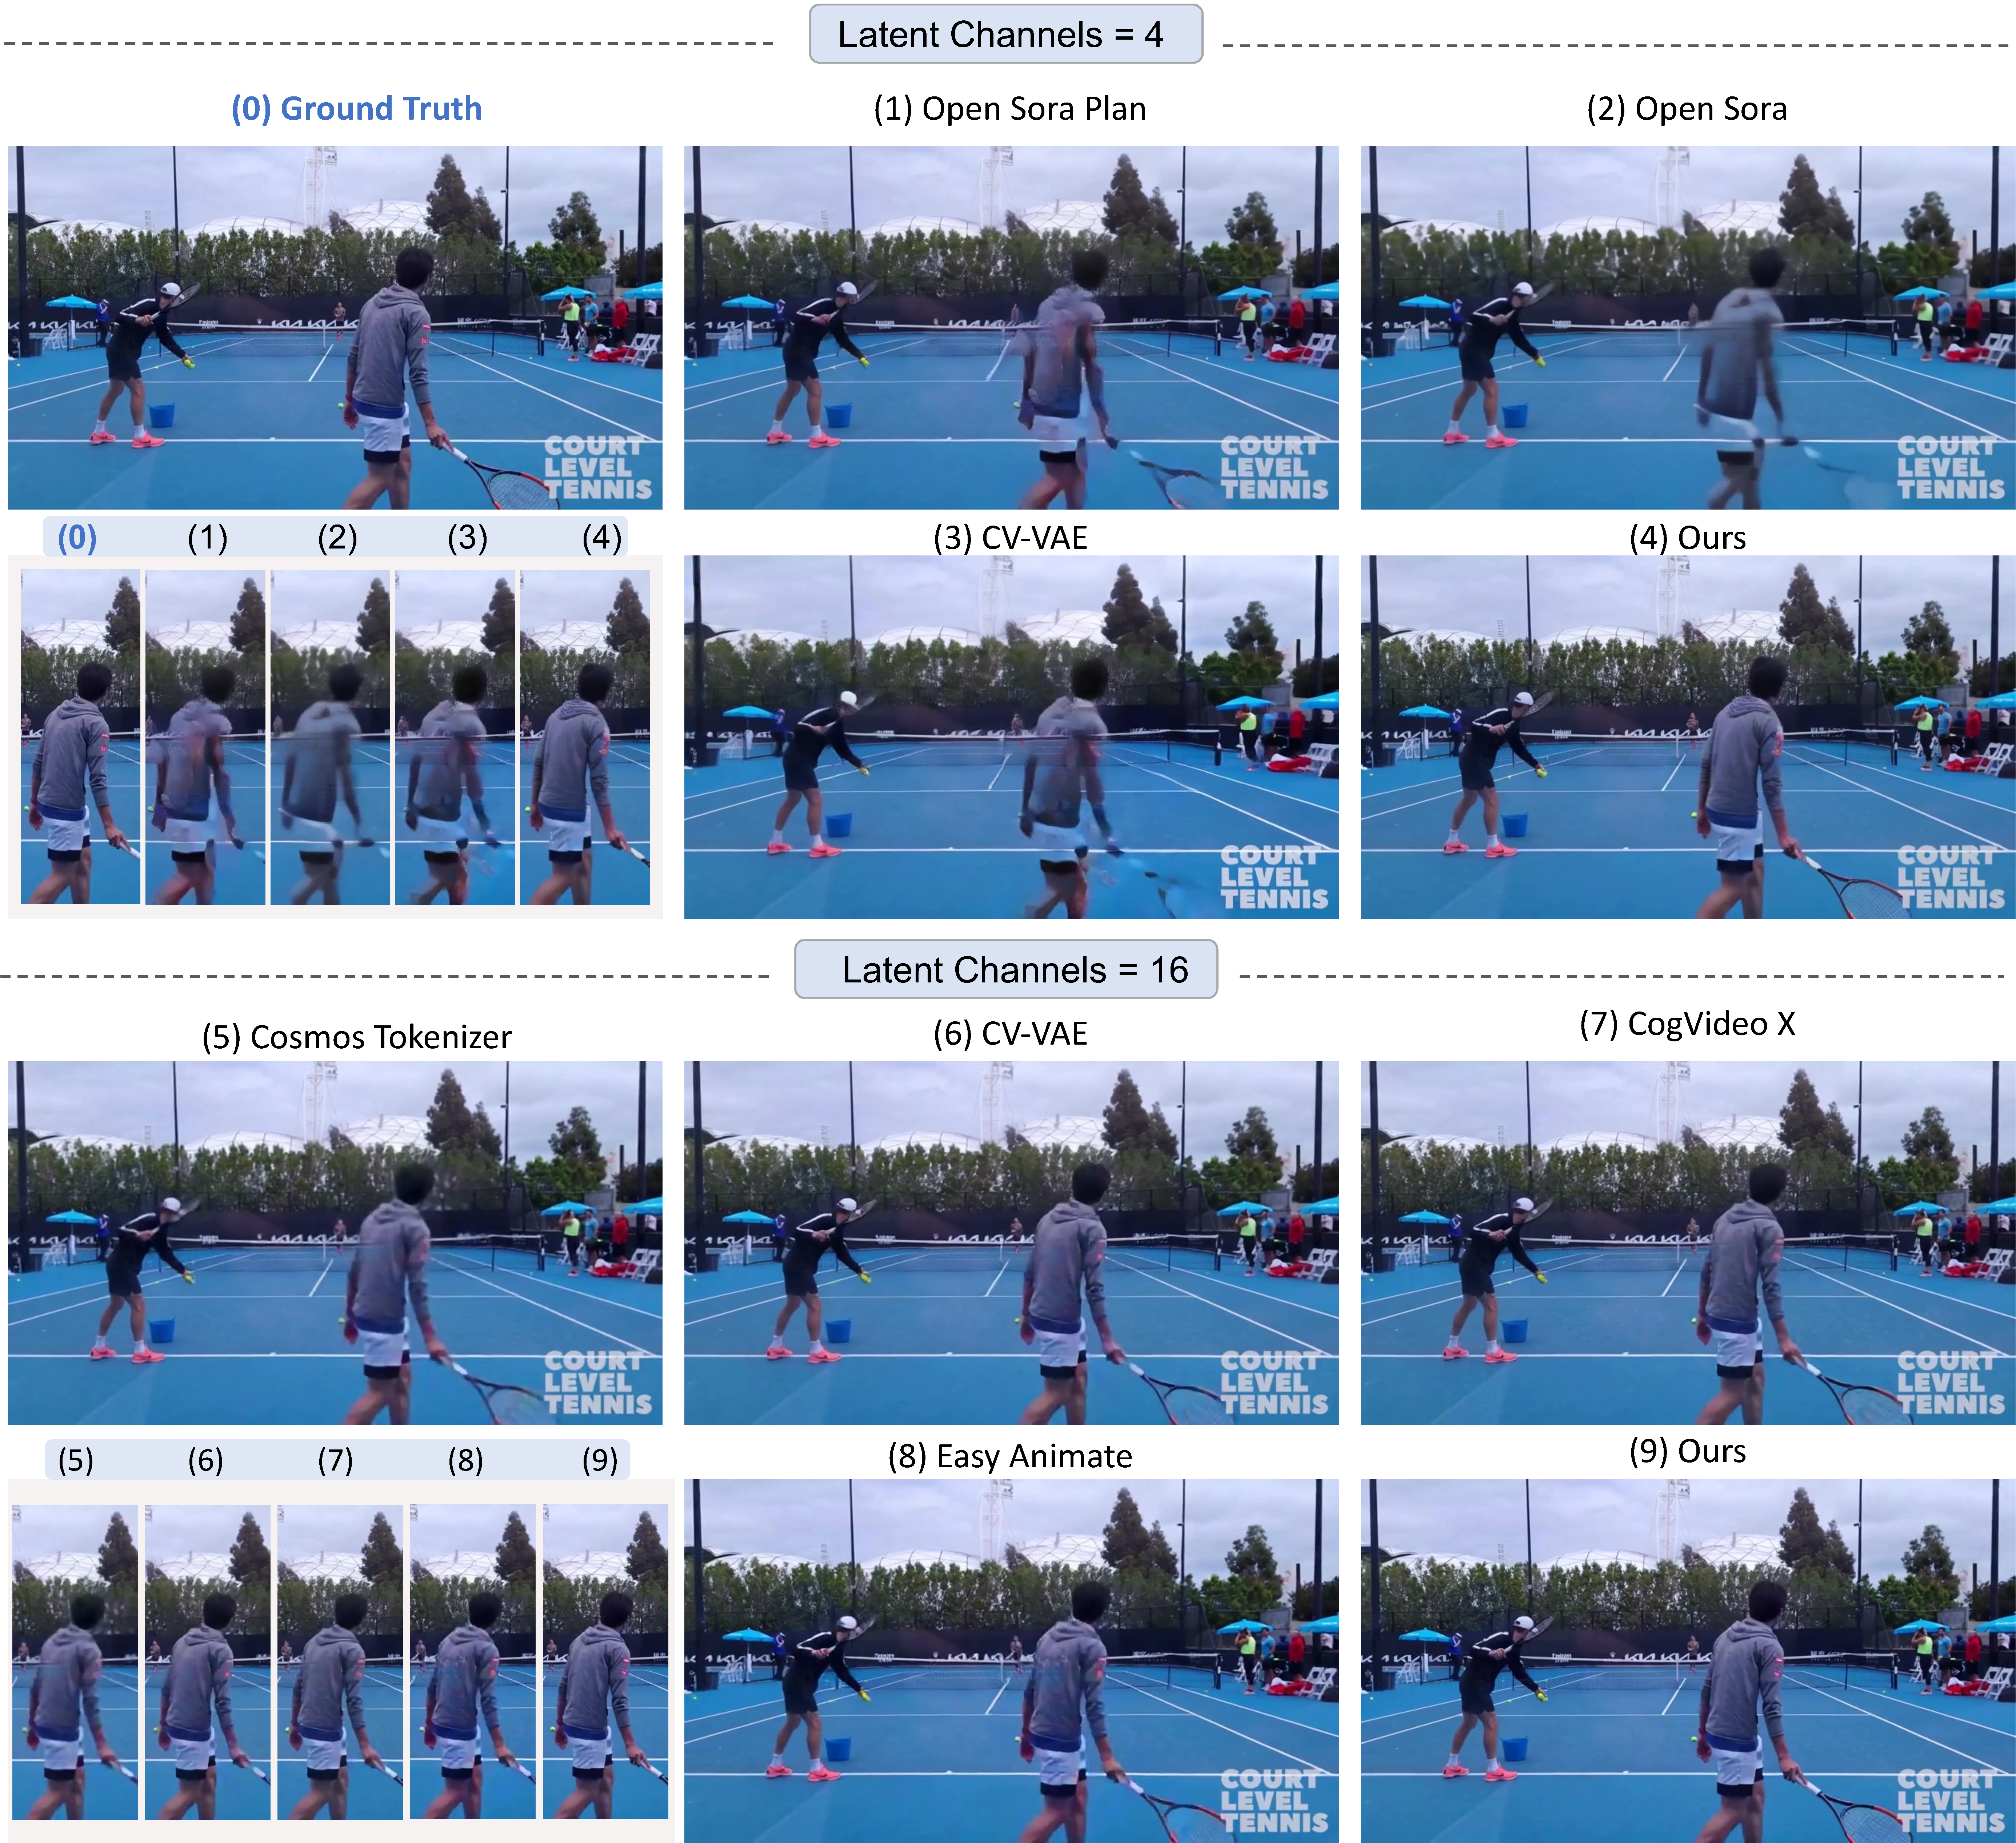
\includegraphics[width=1.0\textwidth]{images/fig1-4and16.pdf}
\caption{
Our reconstruction results compared with a line of three recent strong baseline approaches. 
The ground truth frame is (0). Our model significantly outperforms previous methods, especially under large motion scenarios such as people doing sports.
}
\label{fig:teaser}
\vspace{-3mm}
\end{figure*}



Given the significant attention in the field of video generation, Latent Video Diffusion Models (LVDMs)~\cite{blattmann2023stable, blattmann2023align, he-lvdm, zhou2022magicvideo, he-videocrafter1} have emerged as a popular framework. They have been successfully applied to powerful text-to-video models such as Sora~\cite{videoworldsimulators2024}, VideoCrafter~\cite{he-videocrafter1, chen2024videocrafter2overcomingdatalimitations}, and CogVideoX~\cite{yang2024cogvideox}.
Different from directly generating video pixels, LVDMs generate latent video representations in a compact latent space. This is achieved by first training a Video VAE to encode videos into this latent space.
%
Thus, Video VAE, as a key and fundamental component of LVDMs, has attracted great attention recently.
%
An effective Video VAE can help to reduce the training costs of video diffusion models while improving the final quality of the generated videos.
%
Initially, a series of studies adopt the image VAE from Stable Diffusion~\cite{rombach2022high} for video generation tasks, including AnimateDiff~\cite{guoanimatediff}, MagicVideo~\cite{zhou2022magicvideo}, VideoCrafter1~\cite{he-videocrafter1}, and VideoCrafter2~\cite{chen2024videocrafter2overcomingdatalimitations}. 
%
However, directly adopting an image VAE and compressing video on a frame-by-frame basis leads to temporal flickering due to the lack of temporal correlation. Additionally, the information redundancy along the temporal dimension is not reduced, leading to low training efficiency for subsequent latent video diffusion models.
%
From the introduction of Sora, which compresses videos both temporally and spatially through a Video VAE, a series of studies have emerged that aim to replicate Sora and train their own Video VAEs, including Open Sora~\cite{opensora}, Open Sora Plan~\cite{pku_yuan_lab_and_tuzhan_ai_etc_2024_10948109}, CV-VAE~\cite{zhao2024cv}, CogVideoX~\cite{yang2024cogvideox}, EasyAnimate~\cite{xu2024easyanimatehighperformancelongvideo}, and Cosmos Tokenizer~\cite{cosmos_token}.
%
However, the performance of the current video VAE suffers from many problems, including motion ghost, low-level temporal flickering, blurring (faces, hands, edges, texts), and motion stuttering (lack of correct temporal transition).
% as shown in Fig.~\ref{fig:teaser}.


In this work, we propose a novel cross-modal Video VAE with better spatial and temporal modeling ability in order to solve the aforementioned challenge problems and obtain a robust and high-quality Video VAE.
%
First, we examine different designs for spatial and temporal compression, including simultaneous spatial-temporal (ST) compression and sequential ST compression. 
%
We observed that simultaneous ST compression achieves better low-level temporal smoothness and texture stability, while sequential ST compression achieves better motion recovery, particularly in scenarios of large motion.
%
Thus, we propose a novel architecture that integrates the advantages of both methods and enables effective video detail and motion reconstruction.

Second, we observed that the normally used datasets for text-to-video generation contain text-video pairs. 
Also, during decoding, a text description exists as it serves as the input in the first stage, \textit{i.e.}, the video latent generation stage.
%
To this end, we integrate the text information into the encoding and decoding procedure and propose the first Cross-modal Video VAE.
%
We carefully study how text guidance can be integrated into the spatiotemporal backbone and the mechanism of spatial and temporal semantic guidance. 

In addition, our cross-modal video VAE supports image-video joint training.
To achieve this, we design our network with a fully spatiotemporal factorized architecture, and we feed image and video batches alternately to the network. 
%
During image batches, the data only forwards the spatial part of the network, with the temporal modules being skipped. During video batches, the video forwards both spatial and temporal modules. We also demonstrate that image joint training is crucial for training a video VAE.
%
In summary, our contributions are as follows:
\begin{itemize}
    \item We propose an effective and robust Video VAE, conduct extensive experiments, and achieve the state-of-the-art.
    \item We propose an optimal spatiotemporal modeling approach for Video VAE.
    \item We propose the first cross-modal video VAE that leverages the information from other modalities, i.e., text descriptions, to the best of our knowledge.
    \item Our video VAE is designed and trained to be versatile to conduct both image and video compression. 
\end{itemize}



% \vspace{-2mm}
\section{Related Work}
% \vspace{-2mm}
\label{sec:formatting}
%We now review relevant works on segmentation, vision transformers, and efficient attention.

%-------------------------------------------------------------------------
% \subsection{Video Object Segmentation}
{\bf Video Object Segmentation (VOS)} is a fundamental task in computer vision, segments objects of interest from the background and tracks target objects in a video. 
%Many research works have been proposed in this community on video object segmentation. 
In the unsupervised setting~\citep{grundmann2010efficient,brox2010object,lee2011key,xu2012evaluation,fragkiadaki2012video,perazzi2012saliency,zhang2013video,li2013video,papazoglou2013fast,faktor2014video,wang2015saliency,taylor2015causal,perazzi2016benchmark}, VOS models segment salient objects without a reference mask. In the semi-supervised setting~\citep{pont20172017,xu2018youtube,oh2019video,bhat2020learning,robinson2020learning,li2022recurrent,yang2022decoupling,cheng2022xmem,zhang2023joint,wang2023look,wu2023scalable,cheng2024putting,yang2024scalable}, VOS requires tracking and segmenting objects based on a first-frame mask of target objects. For interactive video object segmentation (iVOS)~\citep{caelles20182018,heo2020interactive,cheng2021modular,homayounfar2021videoclick,yang2023track,cheng2023segment,rajivc2023segment,cheng2024putting,delatolas2024learning}, iVOS models perform object segmentation in videos (masklets) with user guidance, e.g., clicks, bounding boxes, scribbles. In SAM 2~\citep{ravi2024sam}. Semi-supervised VOS and iVOS have been extended to promptable visual segmentation (PVS), where the model can be interactively prompted with different types of inputs such as clicks, boxes, and masks on any frame in a video for segmenting and tracking a valid object.
%-------------------------------------------------------------------------

% \subsection{Vision Transformers}
\noindent {\bf Vision Transformers (ViTs)} have achieved huge success on various vision tasks including image classification~\citep{dosovitskiy2020image}, object detection~\citep{li2022exploring}, image segmentation~\cite{cheng2022masked,kirillov2023segment}, video classification~\citep{fan2021multiscale}, and video object segmentation~\citep{duke2021sstvos,yang2023track}. The original ViT family scales from the efficient ViT-Tiny up to ViT-Huge, with a plain, non-hierarchical architecture. There are also hierarchical vision transformers that combine transformers with hierarchical stage structure, such as Swin~\citep{liu2021swin}, MViT~\citep{fan2021multiscale,li2022mvitv2}, PViT~\citep{wang2021pyramid}, and Hiera~\citep{ryali2023hiera}. While being successful, hierarchical models are usually slower than their plain ViT counterparts for practical deployment~\citep{ryali2023hiera}. 
Combining ViT with convolutions~\citep{lecun1989backpropagation} has been explored for fast hybrid models such as MobileViT~\citep{mehta2021mobilevit}, LeViT~\citep{graham2021levit},  EfficientFormer\citep{li2022efficientformer}, Next-ViT\citep{li2022next}, Tiny-ViT\citep{wu2022tinyvit}, Castling-ViT\citep{you2023castling}, EfficientViT~\citep{liu2023efficientvit}, and MobileNetv4~\citep{qin2024mobilenetv4}. This line of progression towards building efficient ViTs is orthogonal to our
EfficientTAM work towards building efficient video object segmentation. Following SAM~\citep{kirillov2023segment} and EfficientSAMs~\citep{xiong2024efficientsam}, we are pursuing plain ViT backbones for efficient video object segmentation and track anything tasks.  
%The community has also shown increasing interest in efficient vision transformers; \citep{touvron2021training} presented smaller ViTs such as ViT-Small and ViT-Tiny for complementing ViT-Huge, ViT-Large, and ViT-Base in \citep{dosovitskiy2020image}. 


%-------------------------------------------------------------------------
% \subsection{Efficient Attention}
\noindent {\bf Efficient Attention.} The field has developed methods to reduce the quadratic cost of standard self-attention with respect to input sequence length~\cite{attention_is_all_you_need}. 
Local windowed attention has been applied in \cite{beltagy2020longformer,zaheer2020bigbird} for reducing the complexity of self-attention. In \cite{shen2018efficient,katharopoulos-et-al-2020}, a linear dot product approximation is proposed to linearize the softmax matrix in self-attention by heuristically separating keys and queries. In \cite{choromanski2020rethinking}, the Performer model uses random features to approximate self-attention, achieving linear time and memory cost. Nystr\"{o}mformer in \cite{xiong2021nystromformer} makes use of the Nystr\"{o}m method to approximate self-attention with a linear cost. Linformer \cite{wang2020linformer} shows that self-attention is low-rank, which can be approximated by learning linear projection matrices for the keys and values. The approach of~\citep{liu2023efficientvit,you2023castling} leverages the associative property of matrix multiplication for efficient attentions in vision transformers. This direction has shown success and has achieved decent performance on vision tasks. However, in preliminary experiments we found that these methods underperformed in a memory cross-attention module when adapted for efficiency improvement.


%-------------------------------------------------------------------------
% \subsection{Segment Anything Model}
\noindent {\bf Segment Anything Model.} SAM~\citep{kirillov2023segment} is a vision foundation model that can segment any object in an image using interactive prompts such as points and bounding boxes. SAM has demonstrated remarkable zero-shot transfer performance and high versatility for many vision tasks including a broad range of segmentation applications~\citep{chen2023semantic,cen2023sad,deng2023segment,chen2023sam}, in-painting~\citep{yu2023inpaint}, image restoration~\citep{jiang2023restore}, image editing~\citep{gao2023editanything}, image shadow removal~\citep{zhang2023deshadow}, medical image segmentation~\citep{ma2023segment}, camouflaged object detection~\citep{tang2023can}, transparent object detection~\citep{han2023segment}, concept-based explanation~\citep{sun2023explain}, semantic communication~\citep{tariq2023segment}, and object tracking~\citep{cheng2023segment,yang2023track}. The strong ability on image segmentation with flexible prompts motivates the extension of SAM for video object segmentation and track anything. Track Anything Model (TAM)~\citep{yang2023track} combines SAM and XMem~\cite{cheng2022xmem} for interactive video object tracking and segmentation with SAM for frame segmentation and XMem for tracking. SAM-Track~\citep{cheng2023segment} perform object tracking and segmentation in videos by combining SAM~\citep{kirillov2023segment}, DeAOT~\citep{yang2022decoupling}, and Grounding-Dino~\citep{liu2023grounding}. The latest SAM 2~\citep{ravi2024sam} extended SAM for video segmentation through a hierarchical image encoder for frame embeddings and a memory module that conditions current frame embeddings on past frames. Motivated by mobile app use-cases and computationally-constrained applications, recent works have reduced the computational cost of SAM, such as MobileSAM~\citep{zhang2023faster}, FastSAM~\citep{zhao2023fast}, and EfficientSAM~\citep{xiong2024efficientsam}.
The present paper focuses on improving the efficiency challenges of SAM 2 for practical deployment of video object segmentation and track anything.  

\section{Multimodal Image-to-Image Translation}
\label{sec:methods}
Our goal is to learn a multi-modal mapping between two image domains, for example, edges and photographs, or night and day images, etc. 
Consider the input domain $\mathcal{A}\!\subset\!\mathds{R}^{H\!\times W\!\times 3}$, which is to be mapped to an output domain $\mathcal{B}\!\subset\!\mathds{R}^{H\!\times W\!\times 3}$. 
During training, we are given a dataset of paired instances from these domains, $\big\{(\A\!\in\!\mathcal{A}, \B\!\in\!\mathcal{B})\big\}$, which is representative of a joint distribution $p(\A,\B)$.
It is important to note that there could be multiple plausible paired instances $\B$ that would correspond to an input instance $\A$, but the training dataset usually contains only one such pair.
However, given a new instance $\A$ during test time, our model should be able to generate a diverse set of output $\Bh$'s, corresponding to different modes in the distribution $p(\B|\A)$.

While conditional GANs have achieved success in image-to-image translation tasks~\citep{pathakCVPR16context,sangkloy2017scribbler,xian2017texturegan,yang2016high,isola2016image,zhu2017unpaired}, they are primarily limited to generating a deterministic output $\Bh$ given the input image $\A$. 
On the other hand, we would like to learn the mapping that could sample the output $\Bh$ from true conditional distribution given $\A$, and produce results which are both diverse and realistic.
To do so, we learn a low-dimensional latent space $\z \in \mathds{R}^{Z}$, which encapsulates the ambiguous aspects of the output mode which are not present in the input image. For example, a sketch of a shoe could map to a variety of colors and textures, which could get compressed in this latent code. We then learn a deterministic mapping $\G:(\A,\z)\rightarrow \B$ to the output. To enable stochastic sampling, we desire the latent code vector $\z$ to be drawn from some prior distribution $p(\z)$; we use a standard Gaussian distribution $\mathcal{N}(0,I)$ in this work.

We first discuss a simple extension of existing methods and discuss its strengths and weakness, motivating the development of our proposed approach in the subsequent subsections.

\subsection{Baseline: \ppn ($\z \rightarrow \Bh$)}
The recently proposed \pp model~\citep{isola2016image} has shown high quality results in the image-to-image translation setting.
It uses conditional adversarial networks~\citep{goodfellow2014generative,mirza2014conditional} to help produce perceptually realistic results. GANs train a generator $\G$ and discriminator $\D$ by formulating their objective as an adversarial game. The discriminator attempts to differentiate between real images from the dataset and fake samples produced by the generator. Randomly drawn noise $\z$ is added to attempt to induce stochasticity.
We illustrate the formulation in Figure \ref{fig:fig2}(b) and describe it below.
\begin{equation}
\mathcal{L}_{\text{GAN}}(\G,\D) = \mathds{E}_{\A,\B\sim p(\A,\B)}[\log(\D(\A,\B))] + \mathds{E}_{\A\sim p(\A),\z\sim p(\z)}[ \log(1-\D(\A,\G(\A,\z)))]
\label{eqn:Lgan}
\end{equation}

To encourage the output of the generator to match the input as well as stabilize the training, we use an $\ell_1$ loss between the output and the ground truth image.
\begin{equation}
\mathcal{L}_{1}^{\text{image}}(\G) = \mathds{E}_{\A,\B\sim p(\A,\B),\z\sim p(\z)} ||\B - \G(\A,\z) ||_1
\label{eqn:L1}
\end{equation}

The final loss function uses the GAN and $\ell_1$ terms, balanced by $\lambda$. 
\begin{equation}
\G^{*} = \arg\min_{\G} \max_{\D} \quad \mathcal{L}_{\text{GAN}}(\G,\D) + \lambda \mathcal{L}_1^{\text{image}}(\G)
\end{equation}

In this scenario, there is little incentive for the generator to make use of the noise vector which encodes random information.
Isola et al.~\citep{isola2016image} note that the noise was ignored by the generator in preliminary experiments and was removed from the final experiments.
This was consistent with observations made in the conditional settings by~\citep{pathakCVPR16context,mathieu2015deep}, as well as the mode collapse phenomenon observed in unconditional cases~\citep{salimans2016improved,goodfellow2016nips}.
In this paper, we explore different ways to explicitly enforce
%the generator to use the latent encoding, by making it
the latent coding to
capture relevant information.

\subsection{Conditional Variational Autoencoder GAN: \cvaegan ($\B \rightarrow \z \rightarrow \widehat{\mathbf{B}}$)}
One way to force the latent code $\z$ to be ``useful" is to directly map the ground truth $\B$ to it using an encoding function $\E$.
The generator $\G$ then uses both the latent code and the input image $\A$ to synthesize the desired output $\widehat{\mathbf{B}}$.
The overall model can be easily understood as the reconstruction of $\B$, with latent encoding $\z$ concatenated with the paired $\A$ in the middle -- similar to an autoencoder~\citep{hinton2006reducing}. This interpretation is better shown in Figure \ref{fig:fig2}(c).

This approach has been successfully investigated in Variational Autoencoder~\citep{kingma2013auto} in the unconditional scenario without the adversarial objective. Extending it to conditional scenario, the distribution $Q(\z|\B)$ of latent code $\z$ using the encoder $\E$ with a Gaussian assumption, $Q(\z|\B)\triangleq\E(\B)$. To reflect this, Equation \ref{eqn:Lgan} is modified to sampling $\z\sim\E(\B)$ using the re-parameterization trick, allowing direct back-propagation~\citep{kingma2013auto}. 
\begin{equation}
\mathcal{L}_{\text{GAN}}^{\text{VAE}} = \mathds{E}_{\A,\B\sim p(\A,\B)}[\log(\D(\A,\B))] + \mathds{E}_{\A,\B\sim p(\A,\B),\z\sim E(\B)}[ \log(1-\D(\A,\G(\A,\z)))]
\label{eqn:LVAE}
\end{equation}
We make the corresponding change in the $\ell_1$ loss term in Equation \ref{eqn:L1} as well to obtain $\mathcal{L}_1^{\text{VAE}}(\G)=\mathds{E}_{\A,\B\sim p(\A,\B),\z\sim \E(\B)} ||\B - \G(\A,\z) ||_1$. Further, the latent distribution encoded by $E(B)$ is encouraged to be close to a random Gaussian to enable sampling at inference time, when $\B$ is not known.
\begin{equation}
\mathcal{L}_{\text{KL}}(\E) = \mathds{E}_{\B\sim p(\B)} [ \mathcal{D}_{\text{KL}}(\E(\B) || \;\mathcal{N}(0,I)) ],
\label{eqn:KL}
\end{equation}
where $\mathcal{D}_{\text{KL}}(p||q)=-\int  p(z) \log\frac{p(z)}{q(z)}dz $. This forms our \cvaegan objective, a conditional version of the VAE-GAN~\citep{larsen2016vaegan} as
\begin{equation}
\G^{*}, \E^{*} = \arg\min_{\G,\E} \max_{\D}  \quad \mathcal{L}_{\text{GAN}}^{\text{VAE}}(\G,\D,\E)
+ \lambda\mathcal{L}_1^{\text{VAE}}(\G, \E)+\lambda_{\text{KL}}\mathcal{L}_{\text{KL}}(\E).
\end{equation}

As a baseline, we also consider the deterministic version of this approach, i.e., dropping KL-divergence and encoding $\z=E(\B)$.
We call it \cae and show a comparison in the experiments.
There is no guarantee in \cae on the distribution of the latent space $\z$, which makes the test-time sampling of $\z$ difficult. 

% cite cvae-gan
\subsection{Conditional Latent Regressor GAN: \cinfogan ($\z \rightarrow \Bh \rightarrow \zh$)}
We explore another method of enforcing the generator network to utilize the latent code embedding $\z$, while staying close to the actual test time distribution $p(\z)$, but from the latent code's perspective.
As shown in Figure \ref{fig:fig2}(d), we start from a 
% randomly drawn latent code $\z$ and enforce $\E(\G(\A,\z))$ to map back to the same latent code,
randomly drawn latent code $\z$ and attempt to recover it with $\zh=\E(\G(\A,\z))$.
% using an $\ell_1$ loss.
Note that the encoder $\E$ here is producing a point estimate for $\zh$, whereas the encoder in the previous section was predicting a Gaussian distribution.
\begin{equation}
\mathcal{L}_{1}^{\text{latent}}(\G,\E) = \mathds{E}_{\A\sim p(\A),\z\sim p(\z)} ||\z - \E(\G(\A,\z)) ||_1
\label{eqn:L1_lacyc}
\end{equation}

We also include the discriminator loss $L_{\text{GAN}}(\G,\D)$ (Equation \ref{eqn:Lgan}) on $\Bh$ to encourage the network to generate realistic results, and the full loss can be written as:
\begin{equation}
\G^{*}, \E^{*} = \arg\min_{\G,\E} \max_\D \quad \mathcal{L}_{\text{GAN}}(\G,\D) + \lambda_{\text{latent}} \mathcal{L}_1^{\text{latent}}(\G,\E)
\label{fig:L}
\end{equation}

The $\ell_1$ loss for the ground truth image $\B$ is not used. Since the noise vector is randomly drawn, the predicted $\Bh$ does not necessarily need to be close to the ground truth but does need to be realistic. The above objective bears similarity to the ``latent regressor" model~\citep{donahue2016adversarial,dumoulin2016adversarially,xi2016infogan}, where the generated sample $\Bh$ is encoded to generate a latent vector.

\subsection{Our Hybrid Model: \bicycle}
\label{sec:finalMethod}
We combine the \cvaegan and \cinfogan objectives in a hybrid model. For \cvaegan, the encoding is learned from real data, but a random latent code may not yield realistic images at test time -- the KL loss may not be well optimized. Perhaps more importantly, the adversarial classifier $\D$ does not have a chance to see results sampled from the prior during training. 
%  latent space may not be organized in an easy manner to be sampled from
In \cinfogan, the latent space is easily sampled from a simple distribution, but the generator is trained without the benefit of seeing ground truth input-output pairs. We propose to train with constraints in both directions, aiming to take advantage of both cycles ($\B \rightarrow \z \rightarrow \widehat{\mathbf{B}}$ and $\z \rightarrow \Bh \rightarrow \zh$), hence the name \bicycle.

\vspace{-3mm}
\begin{equation}
\begin{split}
\G^{*}, \E^{*} = \arg\min_{\G,\E} \max_{\D} \quad  & \mathcal{L}_{\text{GAN}}^{\text{VAE}}(\G,\D,\E) + \lambda \mathcal{L}_1^{\text{VAE}}(\G,\E) \\
+& \mathcal{L}_{\text{GAN}}(\G,\D) + \lambda_{\text{latent}} \mathcal{L}_1^{\text{latent}}(\G,\E) + \lambda_{\text{KL}}\mathcal{L}_{\text{KL}}(\E),
\end{split}
\label{eq:L}
\end{equation}
where the hyper-parameters $\lambda$, $\lambda_{\text{latent}}$, and $\lambda_{\text{KL}}$ control the relative importance of each term. 

In the unconditional GAN setting, \citet{larsen2016vaegan} observe that using samples from both the prior $\mathcal{N}(0,I)$ and encoded $\E(\B)$ distributions further improves results.
Hence, we also report one variant which is the full objective shown above (Equation~\ref{eq:L}), but without the reconstruction loss on the latent space $\mathcal{L}_1^{\text{latent}}$. 
We call it \cvaeganp, as it is based on \cvaegan with an additional loss $\mathcal{L}_{\text{GAN}}(G, D)$, which allows the discriminator to see randomly drawn samples from the prior.
\vspace{-2mm}

\section{Implementation Details}
\label{sec:implementation}
The code and additional results are publicly available at \url{https://github.com/junyanz/BicycleGAN}. Please refer to our website for more details about the datasets, architectures, and training procedures.
\begin{figure}
\centering
% \hspace{-.08\linewidth}
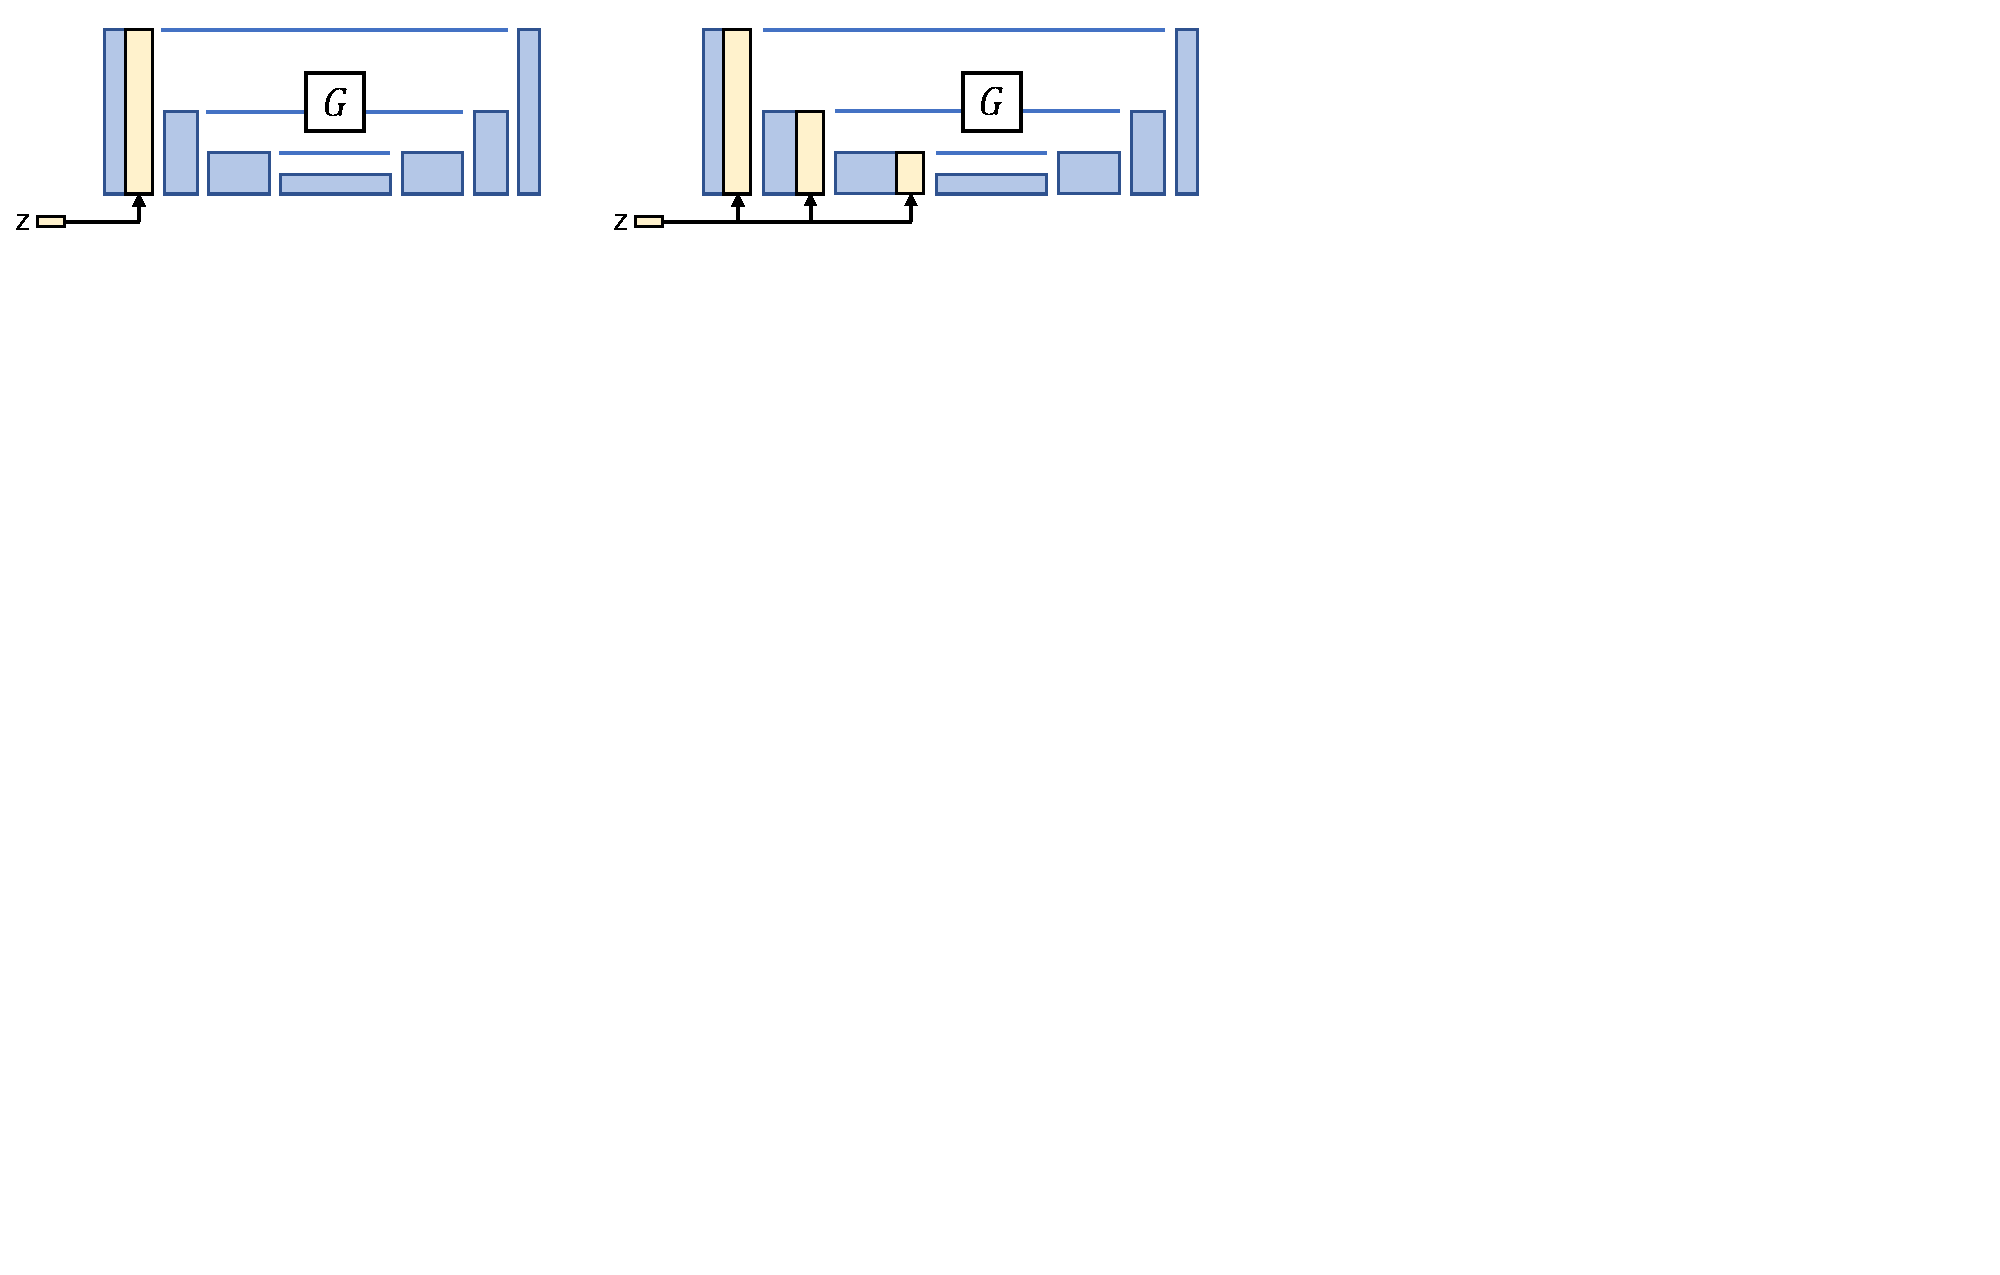
\includegraphics[width=1.0\linewidth]{imgs/injectz.pdf}
\caption{\small \textbf{Alternatives for injecting {\bf z} into generator.} Latent code \textbf{z} is injected by spatial replication and concatenation into the generator network. We tried two alternatives, {\bf (left)} injecting into the input layer and {\bf (right)} every intermediate layer in the encoder.}
\vspace{-4mm}
\label{fig:addz}
\end{figure}

\paragraph{Network architecture} For generator $\G$, we use the U-Net~\citep{ronneberger2015u}, which contains an encoder-decoder architecture, with symmetric skip connections. The architecture has been shown to produce strong results in the unimodal image prediction setting when there is a spatial correspondence between input and output pairs. For discriminator $\D$, we use two PatchGAN discriminators~\citep{isola2016image} at different scales, which aims to predict real vs. fake for $70\times 70$ and $140 \times 140$ overlapping image patches. For the encoder $\E$, we experiment with two networks: (1) \texttt{E\textsubscript{CNN}}: CNN with a few convolutional and downsampling layers and (2) \texttt{E\textsubscript{ResNet}}: a classifier with several residual blocks~\cite{he2016deep}.

\paragraph{Training details} We build our model on the Least Squares GANs (LSGANs) variant~\citep{mao2016least}, which uses a least-squares objective instead of a cross entropy loss. LSGANs produce high-quality results with stable training. We also find that not conditioning the discriminator $\D$ on input $\mathbf{A}$ leads to better results (also discussed in~\citep{pathakCVPR16context}), and hence choose to do the same for all methods. We set the parameters $\lambda_{\text{image}}=10$, $\lambda_{\text{latent}}=0.5$ and $\lambda_{\text{KL}}=0.01$ in all our experiments. We tie the weights for the generators and encoders in the \cvaegan and \cinfogan models. For the encoder, only the predicted mean is used in \cinfogan. We observe that using two separate discriminators yields slightly better visual results compared to sharing weights. We only update $\G$ for the $\ell_1$ loss $\mathcal{L}_{1}^{\text{latent}}(\G,\E)$ on the latent code (Equation \ref{eqn:L1_lacyc}), while keeping $\E$ fixed. We found optimizing $\G$ and $\E$ simultaneously for the loss would encourage $G$ and $E$ to hide the information of the latent code without learning meaningful modes.
We train our networks from scratch using Adam~\citep{kingma2014adam} with a batch size of $1$ and with a learning rate of $0.0002$. We choose latent dimension $|\z|=8$ across all the datasets. 

{\bf Injecting the latent code $\z$ to generator}.
We explore two ways of propagating the latent code $\z$ to the output, as shown in Figure~\ref{fig:addz}: 
(1) \texttt{add\_to\_input}: we spatially replicate a $Z$-dimensional latent code $\z$ to an $H\!\times W\!\times Z$ tensor and concatenate it with the $H\!\times W\!\times 3$ input image and (2)~\texttt{add\_to\_all}: we add $\z$ to each intermediate layer of the network $\G$, after spatial replication to the appropriate sizes.

\vspace{-1mm}

\section{Experiments}

\subsection{Experimental setup}

Our experiments all use the Llama \citep{Llama} architecture trained on WikiText-103~\citep{WikiText103} (excepting the large-scale runs in \Cref{sec:fp8_training}). We apply current best-practice LLM training techniques from the literature (full settings are given in \Cref{tab:experiment_defaults}). In accordance with our analysis of settings for \mut\ in \Cref{sec:challenges:mut}, we remove parameters from norm layers, use independent AdamW, and avoid training on too many epochs for both \umup\ and \mup\ for the sake of fair comparison.

\subsection{Quantifying hyperparameter interdependence} \label{sec:experiments:hp_independence}

Our principled approach to HPs (\Cref{sec:umup:principled_hps}) contains the requirement that their optimal values should depend minimally on the value of other HPs. We now investigate this empirically, conducting a 2D sweep over every pair of HPs for \mup\ and \umup, shown in \Cref{fig:additional_experiments:mult_grid_mup,,fig:additional_experiments:mult_grid_umup} respectively.

To derive an empirical measure of HP dependency, we introduce the notion of \textit{transfer error} (see \Cref{alg:transfer_error}). This considers a pair of HPs, with one `fixed' and the other for `transfer'. We take the best value of the transfer HP for each non-optimal value of the fixed HP, and use it with the optimal value of the fixed HP. The transfer error is the difference between the losses obtained and the minimum loss. \Cref{fig:experiments:transfer_error} shows this measure for each pair of HPs under \mup\ and \umup, reflecting the improvement in HP dependency as a result of our scheme. This gives \umup\ a reduced risk of small transfer errors leading to large degradations, and the potential to sweep HPs in a more separable way.

\begin{figure}[t]
    \vspace{-1em}
    \centering
    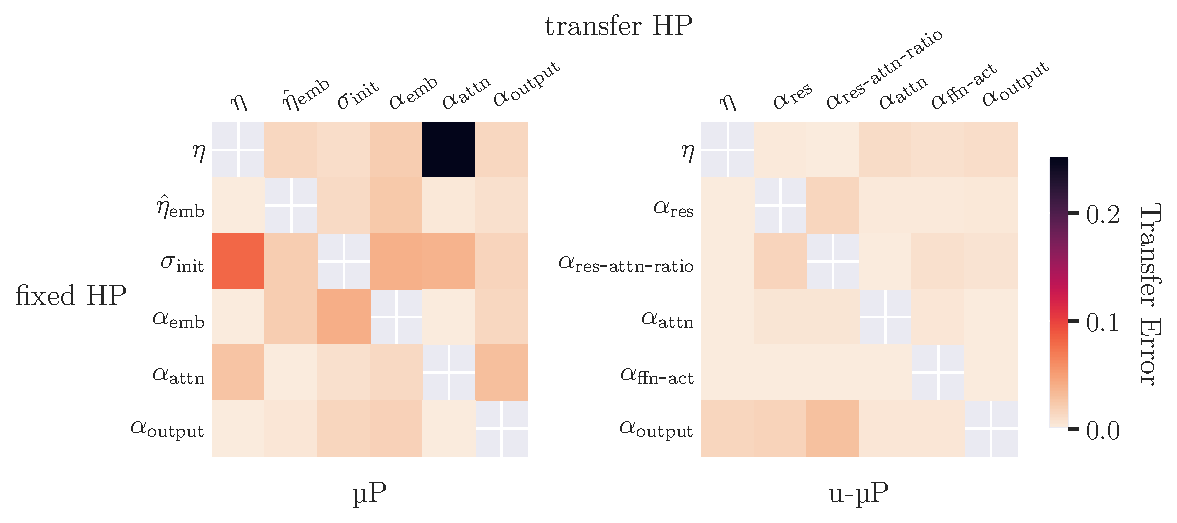
\includegraphics[width=\textwidth]{arXiv/figures/hp_pair_dependencies_val.pdf}
    \caption{A visualization of the dependencies between pairs of HPs under each scheme. Transfer error measures the extent to which the optimal value of the transfer HP depends on the fixed HP (see \Cref{alg:transfer_error}). On average, \mup\ has a transfer error of 0.03, whereas \umup\ has 0.005.}
    \label{fig:experiments:transfer_error}
\end{figure}

\subsection{Hyperparameter search} We now leverage this improved separability of HPs for the purpose of efficient sweeping. In \Cref{fig:fig1}~(a) we conduct a standard random search for \mup\ and \umup, along with the independent search outlined in \Cref{sec:umup_hp_search} (and \Cref{app:umup_hp_search_algorithm}). We observe the following:

\begin{enumerate}
    \item For \umup\ the LR-sweep phase of independent search alone is sufficient to reach near-optimal loss (totaling 9 runs). During this phase other HPs are fixed at 1, which for \umup\ means that the inputs to operations are generally unit-scaled.

    \item Consequently, we conclude that unit scale at initialization is close to the ideal scaling for effective learning here. This is not a property we asserted a priori, nor do we argue that it necessarily holds for other training setups and models; hence why we still provide a set of extended HPs to be swept.

    \item In contrast \mup\ still requires non-LR HPs to be swept to attain a reasonable loss. Unlike \umup, fixing HPs at 1 results in arbitrarily-scaled inputs, which appear to result in worse training.

    \item The `combined mults' phase causes the loss to spike for \mup. This is due to the HP dependencies shown in \Cref{fig:experiments:transfer_error}, which mean HPs cannot be swept independently and used together. Conversely, lower dependence means this can be done for \umup, making random search unnecessary.
\end{enumerate}

\subsection{Hyperparameter transfer}

% As \umup\ follows the \mup\ parametrization rules (with the exception of the embedding LR scaling rule in \Cref{sec:umup:emb_lr_rule}), we still expect it to satisfy the transfer properties of \mup. In fact, \umup's transfer properties are generally better than those of the \mup\ baseline, thanks to our unit-scale criterion and careful HP design.

We demonstrate the transfer of LR across width in \Cref{fig:fig1} (b), of the other extended HPs across width in \Cref{fig:lr_transfer}, and of LR across training steps, batch size and depth in \Cref{fig:experiments:hp_transfer_over_width}. We find that:

\begin{enumerate}
    \item The optimal LR is constant for all widths under \umup, from 128 to 4096.

    \item The optimal LR is also approximately constant for training steps, batch size and depth. This means we can scale our proxy model down across all these axes and maintain LR transfer. Of these, width appears the most stable and depth the least.

    \item Whereas \mup\ sees diminishing returns for larger widths, \umup\ continues to benefit from width, with the 2048 \umup\ model matching the 4096 \mup\ model. We attribute this primarily to our improved embedding LR rule.

    \item Non-LR HPs also have approximately constant optima across width under \umup. This is not true for \mup, where $\hat{\eta}_\mathrm{emb}$ has poor transfer due to the embedding scaling rule issue identified in \Cref{sec:umup:emb_lr_rule}, along with $\sigma_\mathrm{init}$ which in \Cref{sec:challenges:which_hps} we argue should not be grouped across all weights (and drop from the \umup\ HP scheme).

    \item The optimal values found for non-LR HPs are all close to 1. In practice this means that dropping these HPs entirely is potentially viable for similar models and training setups.
\end{enumerate}

\begin{figure}[t]
    \centering
    \begin{subfigure}{\textwidth}
        \centering
        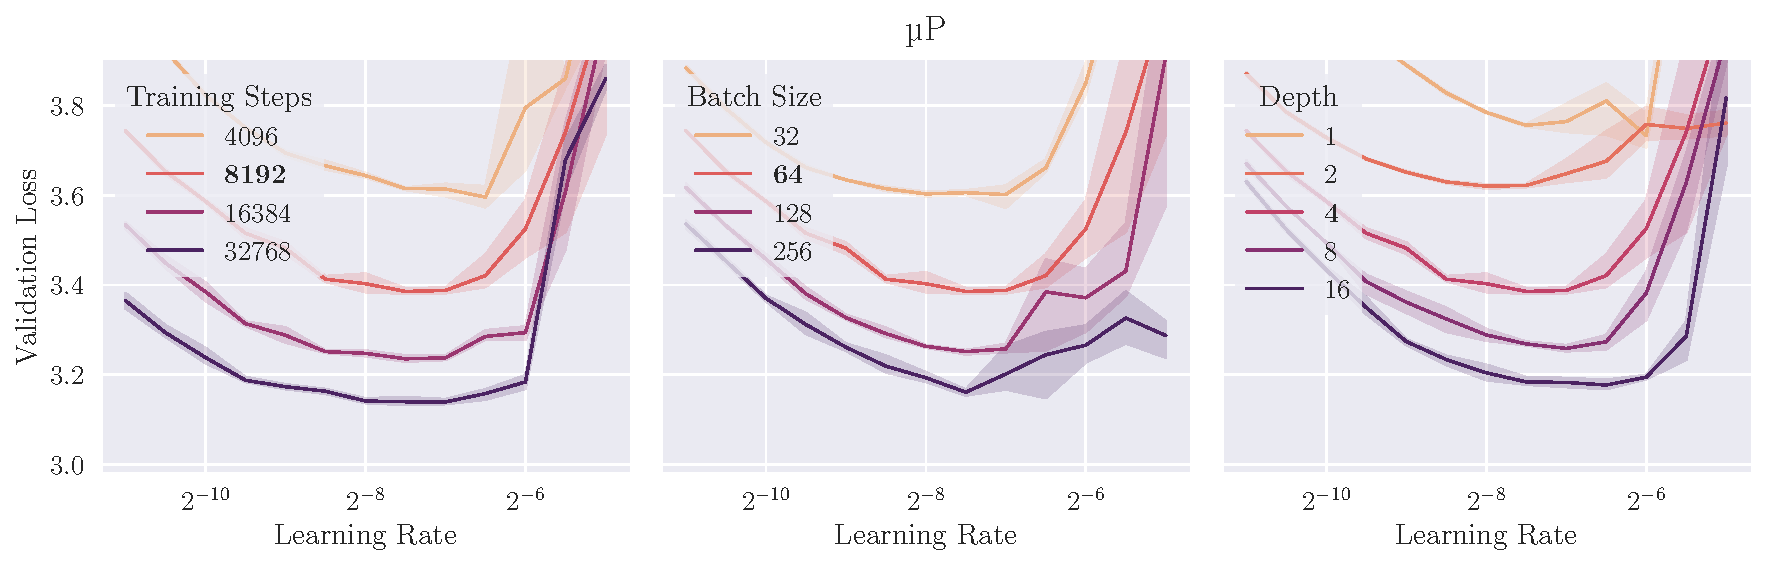
\includegraphics[width=\textwidth]{arXiv/figures/lr_transfer_mup.pdf}
    \end{subfigure}
    \begin{subfigure}{\textwidth}
        \centering
        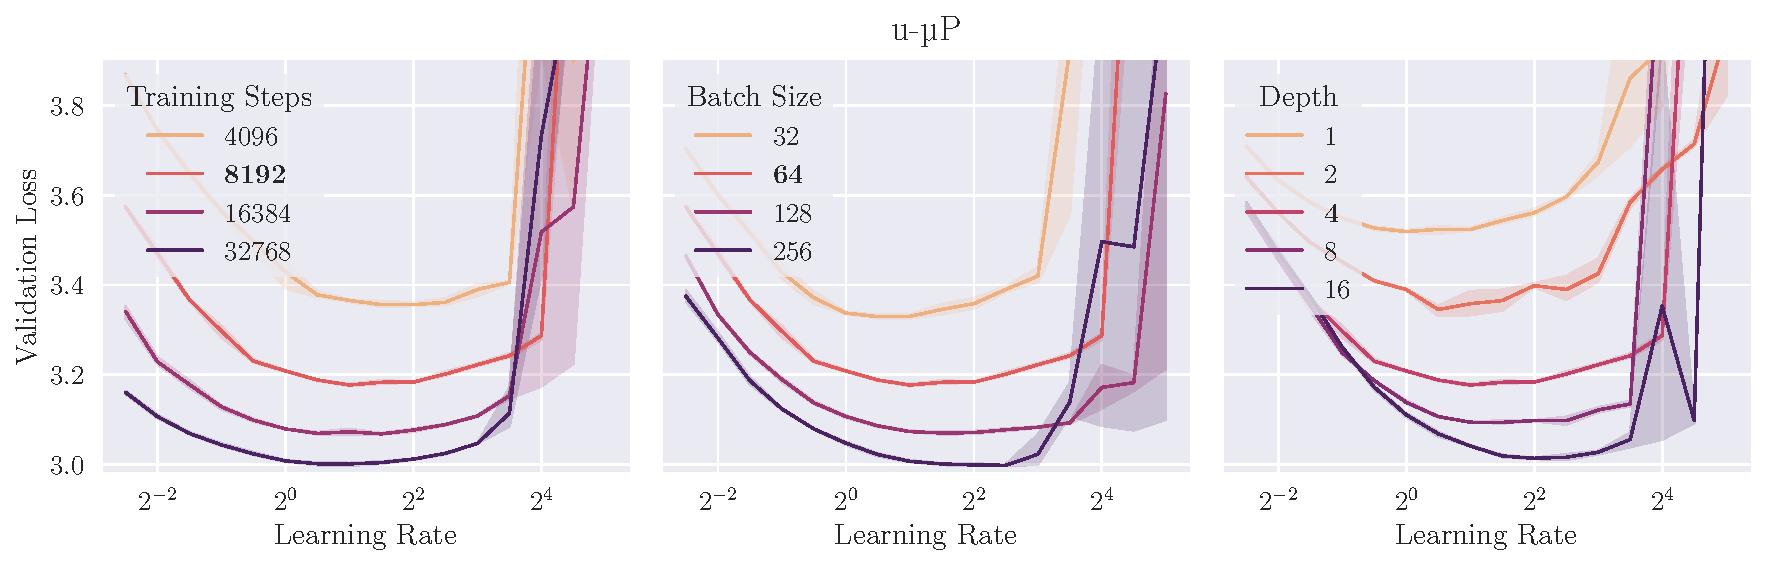
\includegraphics[width=\textwidth]{arXiv/figures/lr_transfer_u-mup.pdf}
    \end{subfigure}
    \caption{Learning rate transfer for \mup{} (top) and \umup{} (bottom), over training steps, batch size and depth. See \Cref{fig:fig1}~(b) for transfer over width. The \textbf{default} shape parameter for other panels is shown in bold. The shaded area shows the $95\%$ confidence interval for the mean.}
    \label{fig:lr_transfer}
\end{figure}

\subsection{FP8 training} \label{sec:fp8_training}

In this section we justify the simple mixed-precision scheme described in \Cref{sec:umup:low_prec_training} and demonstrate that it can be used to train \umup\ models out-of-the-box.

\paragraph{Proof-of-concept} \Cref{fig:numerics:scale} shows the RMS of all linear layer inputs for a moderately sized transformer. RMS captures the larger of the mean and scale of a distribution, and as such is a good test of whether a tensor is likely to suffer over/underflow in low-precision. We observe that \umup\ tensors largely have RMS starting close to $1$ and remaining so at the end of training, supporting our scheme.

\Cref{fig:numerics:rms_during_training} demonstrates the scale-growth of critical tensors which our scheme is designed to accommodate, showing RMS on a per-tensor basis over steps. \Cref{fig:numerics:scale_scaling} provides further insight into this issue, showing the effect of LR, width, depth, steps and batch size on the RMS of critical tensors.

As an initial proof-of-concept we train a \umup\ model using our FP8 scheme over 8k steps, using HPs from a proxy model, as shown in \Cref{fig:fig1}~(c). We see only a small degradation versus FP32, and at this scale critical tensors can still be cast to FP8 using \texttt{E5M2}, while gradients can even use \texttt{E4M3}.

%\subsection{Numerical properties} \label{subsec:numerical_properties}

%,  Detailed analysis of these statistics is given in \Cref{app:fp8_training}, with our results supporting the central thesis of Unit Scaling: that tensors are well-scaled at initialization and largely remain so across training.

%Based on these conclusions we propose our primary FP8 scheme: for every matrix multiplication, we cast the input, weight and grad-output tensors to \texttt{E4M3}, with the exception of the inputs to FFN and self-attention final projections, which are cast to \texttt{E5M2} to accommodate their growing scale. This simply requires FP8 casts to be inserted into the model, avoiding the more complex scaling techniques used for FP8 in the literature (see \Cref{app:low_precision_and_its_trade_offs}). This is possible due to the numerical stability we see in our analysis of \umup. Additional details of our primary FP8 scheme are given in \Cref{app:fp8_scheme}.

%As we demonstrate in \Cref{subsec:large_scale}, the primary scheme needs to be slightly adapted when model size, sequence length and number of training steps increase substantially. 

%\subsection{FP8 training at smaller scale} \label{sec:experiments:fp8}

%We now show that \umup\ can indeed be trained in our primary FP8 scheme in a smaller-scale setting (in terms of training tokens, rather than model-size). We note that our aim here is a proof-of-concept that this form of low-precision training can be done without degradation, not a demonstration of improved throughput which we leave to future work. To investigate the question of the potential benefits of FP8 training, \Cref{app:scaled_mm_benchmarking} shows results for micro-benchmarking low-precision matmuls. We find that the addition of scaling factors adds no overhead, making our \umup\ modifications essentially `free'.

%\Cref{fig:fig1} (c) demonstrates the application of our FP8 scheme to model-training at width 4096. We use exactly the HPs suggested by the sweep in \Cref{fig:fig1} (a), but transferred to the larger model-width. \mup\ fails entirely under our FP8 scheme due to gradient underflow, reflecting the requirement for different, and likely more complex scaling scheme. In contrast, \umup\ trains in FP8 with only a small increase in validation loss versus the full-precision baseline.

\begin{figure}[t]
    \centering
    \begin{subfigure}{.46\textwidth}
        \centering
        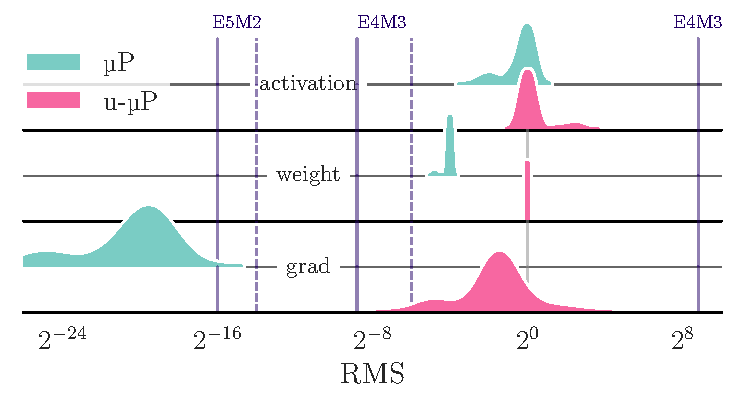
\includegraphics[width=\textwidth]{arXiv/figures/rms_at_init.pdf}
    \end{subfigure}
    \begin{subfigure}{.46\textwidth}
        \centering
        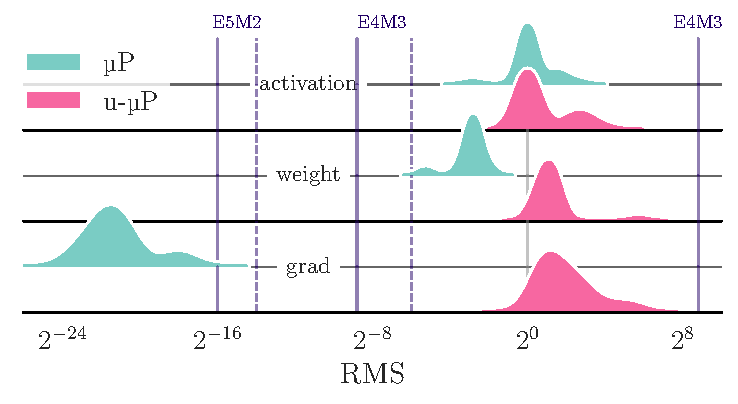
\includegraphics[width=\textwidth]{arXiv/figures/rms_end_training.pdf}
    \end{subfigure}
    \caption{Per-tensor $\mathrm{RMS} = \sqrt{\sigma^2 + \mu^2}$ across \umup\ and \mup\ models at initialization (left) and after training (right). \umup\ tensors have RMS that starts close to $1$ and remains within E4M3 range at the end of training. Dashed and solid red lines show each format's min. normal and subnormal values.}
    \label{fig:numerics:scale}
\end{figure}

%\subsection{FP8 training at large-scale} \label{subsec:large_scale}

\paragraph{Larger scale} Next we consider a more realistic training scenario \footnote{The training codebase used for our larger-scale experiments can be found at the following url \url{https://github.com/Aleph-Alpha/scaling}. We have also released model checkpoints, which are available at \url{https://huggingface.co/Aleph-Alpha}.}.
% \footnote{The large scale experiments were run on a separate code base optimized for distributed training that will be made available in the near future.}
Using the same architecture, and following the steps set out in our \umup\ user-guide (\Cref{app:using_umup_guide}), we train our target models on 300B tokens of the SlimPajama dataset \citep{SlimPajama} (see \Cref{app:large_model_training} for training details).

We begin with an independent search (\Cref{sec:umup_hp_search}) over our \umup\ proxy model's HPs. Here we make the following observations:
\begin{enumerate}
    \item When using a relatively small proxy model (8 layers and 512 width), the HP-loss landscape is rather noisy. By doubling the width we can discern optimal HP values more clearly.
    \item The most important HPs are $\eta$ and $\alpha_\mathrm{res\text{-}attn\text{-}ratio}$. All others can be left at the default of $1$.
    \item The optimal values of these HPs are $\eta = 2^{3.5}$ and $\alpha_\mathrm{res\text{-}attn\text{-}ratio} = 2^{-2.0}$ and thus differ non-trivially from the observed HPs in our smaller-scale experiments.
\end{enumerate}

We then train \umup\ models of approximately 1B, 3B and 7B parameters, using our FP8 mixed-precision scheme (see \Cref{sec:umup:low_prec_training}). We also train two baselines at each size: the first is a BF16 version of our \umup\ models, and the second is a set of SP models using the weight init scheme from the Pythia model family~\citep{Pythia} and the LR scheme from Llama 3~\citep{LLAMA3}, scaling inversely with width and using a LR of 3e-4 at 7B scale.
The loss curves are shown in \Cref{fig:scaleup}. All FP8 runs converge and show no significant loss degradation. In comparison to SP, the \umup\ models have a qualitatively different training curve with a higher loss for most of training that catches up in latter stages, hinting at a fundamentally different optimization trajectory. In terms of downstream performance, both of the \umup\ 7B models are competitive with SP. In particular, the scores of the FP8 model are mostly on par with the BF16 models (see \Cref{tab:eval_results}).

%We also record the magnitude of tensors in the model during training (\ce{TODO: include figure }). Some of the critical layers show a significant scale growth over time, which makes it impossible to naively cast them to FP8. On the other hand, the non-critical tensor scales are very stable across training time, and model size. This is strong evidence for \umup\ FP8 to work at even larger scales.

% . We also observe that using purely the \texttt{E4M3} format in the `non-problematic' layers leads to divergence as well, whereas the hybrid scheme of using \texttt{E4M3} for the activation and the weight and \texttt{E5M2} for the output gradient is stable.
%To tackle the layers that exhibit scale growth, we fit them with a lightweight form of dynamic rescaling, leaving the rest of the model untouched. 

%The dynamic rescaling works as follows: Before the matrix multiplication, we normalize the input by its standard deviation and divide the result by the same scale afterwards, while ignoring both of these operations in the backward computation. We emphasize that this is still considerably less complex than the per-tensor scaling strategy that is usually required for FP8 training.

%Using this refined FP8 scheme we perform two series of experiments:
%\begin{enumerate}
  %  \item On the 1B scale, we train a comparable SP model adopting the learning rate and initialization scheme from the Pythia model family~\citep{Pythia}, which we consider a strong established baseline. Apart from a standard training in BF16 mixed precision, we also try a simple FP8 cast and the Nvidia Transformer Engine framework~\citep{Transformer_Engine} for this baseline. We then compare these SP models to three variants of our \umup\ 1B model: One model in mixed precision, one model casting all layers except the critical ones to FP8 (our `partial' scheme in \Cref{fig:scaleup}), and one where we apply our full FP8 scheme. Overall the \umup\ models perform favorably  (see \Cref{fig:scaleup} (left)).
   % \item We train FP8 models up to 7B parameters using our full FP8 scheme. All runs converge (see \Cref{fig:scaleup} right), and we expect our method to work at larger scales still.
%\end{enumerate}


%We then train our target models using this FP8 scheme in \Cref{fig:dynamic_rescaling_losses}. At each model-size we demonstrate successful FP8 training, and expect it to work at larger scales still.

%\begin{figure}[t]
  %  \centering
  %  \begin{subfigure}{\textwidth}
  %      \centering
  %      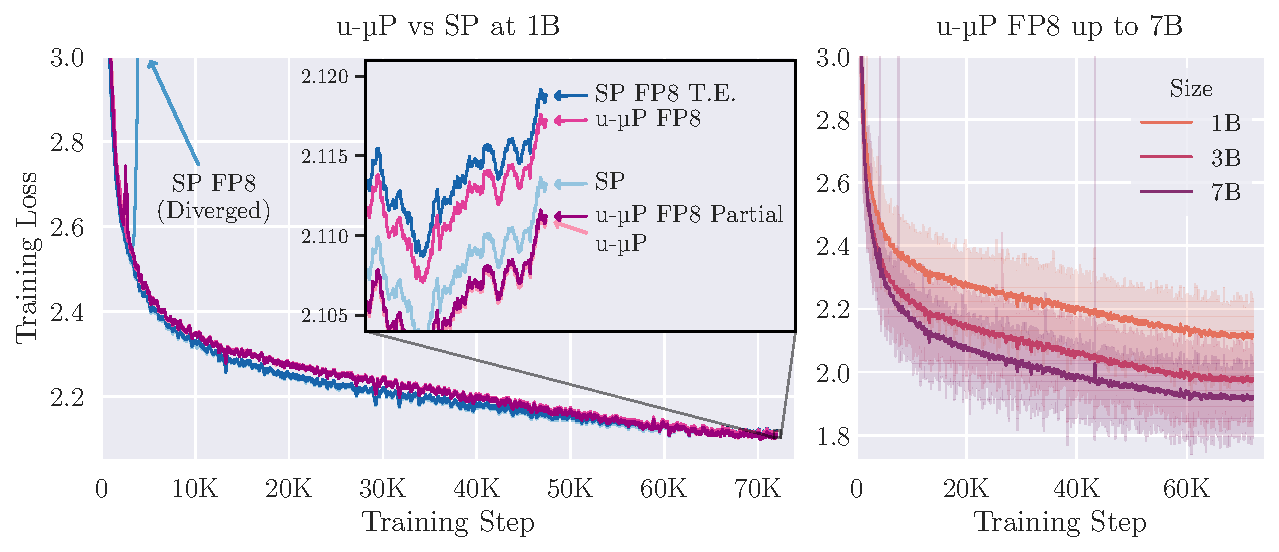
\includegraphics[width=\textwidth]{arXiv/figures/fig_scaleup.pdf}
  %  \end{subfigure}
  %  \caption{(Left) Comparison of 1B training curves for \umup\ and SP, using BF16 mixed precision vs FP8. Directly casting to FP8 causes SP to diverge, whereas \umup\ still converges and outperforms the Transformer Engine FP8 baseline (SP FP8 T.E.). Using our proposed partial FP8 scheme, \umup\ maintains nearly full performance compared to BF16 mixed precision. (Right) Loss curves from large scale training runs up to 7B using the \umup\ FP8 scheme. Both figures use a smoothed running average loss with window size 100.}
  %  \label{fig:scaleup}
%\end{figure}

\begin{figure}[t]
    \vspace{-1.5em}
    \centering
    \begin{subfigure}{0.4\textwidth}
        \centering
        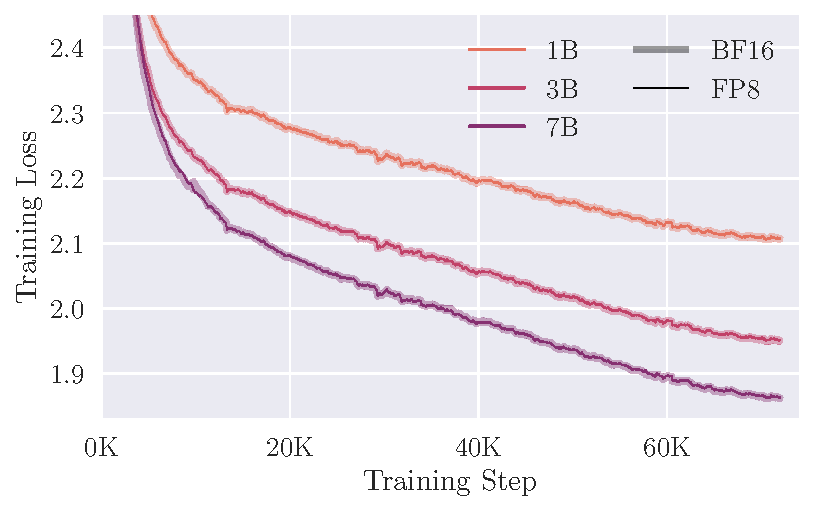
\includegraphics[width=\textwidth]{arXiv/figures/large_scale_BF16_vs_FP8.pdf}
    \end{subfigure}
    \hspace{2em}
    \begin{subfigure}{0.4\textwidth}
        \centering
        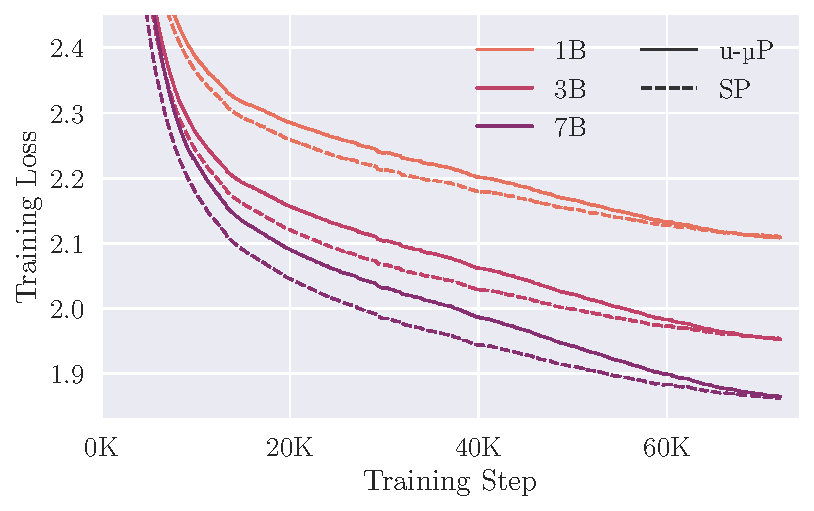
\includegraphics[width=\textwidth]{arXiv/figures/large_scale_umup_vs_sp.pdf}
    \end{subfigure}
    \vspace{-0.5em}
    \caption{Large-scale training runs. (Left) \umup\ BF16 vs \umup\ FP8. (Right) \umup\ BF16 vs SP BF16.}
    \label{fig:scaleup}
\end{figure}

\begin{table}[t] 
  \centering
  \caption{0-shot benchmark results at 7B scale.}
\begin{tabular}{llcccccc}
\toprule
Scheme & Format & MMLU & HellaSwag & OpenBook QA & PIQA & TriviaQA & WinoGr \\
\midrule
SP & BF16 & 29.6 & 52.4 & 27.8 & 76.5 & 22.2 & 63.3 \\
\umup\ & BF16 & 29.0 & \textbf{53.4} & \textbf{31.6} & 77.1 & \textbf{23.4} & 63.7 \\
\umup\ & FP8 & \textbf{31.2} & \textbf{53.4} & 29.6 & \textbf{77.6} & 21.3 & \textbf{65.7} \\
\bottomrule
\label{tab:eval_results}
\vspace{-1.5em}
\end{tabular}
\end{table}




  %To a Results for this can be seen in \todocite. We observe a small benefit in using non-unit values for the $\mathord{?}$ and $\mathord{?}$ HPs, as well as a slightly different optimal LR ($\mathord{?}$ instead of $2^{1.5}$).

%Transferring these HPs to our target models, we train SP and \umup\ models at the 1B, 3B and 7B scale, with and without FP8, as shown in figure \todocite. Using our transferred HPs, our \umup\ models match the SP baselines, and unlike the SP models can be trained using a simple FP8 scheme. This differs slightly from our primary FP8 scheme as the two activation tensors that exhibit scale-growth require dynamic scaling (see \Cref{app:large_model_training}), though the large majority of tensors still use our un-scaled FP8 cast. This demonstrates that our scheme can be applied effectively to LLMs in realistic training settings.

%[add any additional details here, and to corresponding Appendix A section once figures are ready]


\section{Conclusions}
\label{sec:conclusion}
\vspace{-2mm}

In conclusion, we have evaluated a few methods for combating the problem of mode collapse in the conditional image generation setting. We find that by combining multiple objectives for encouraging a bijective mapping between the latent and output spaces, we obtain results which are more realistic and diverse. We see many interesting avenues of future work, including directly enforcing a distribution in the latent space that encodes semantically meaningful attributes to allow for image-to-image transformations with user controllable parameters.


{\bf Acknowledgments}
\small We thank Phillip Isola and Tinghui Zhou for helpful discussions. 
This work was supported in part by Adobe Inc., DARPA, AFRL, DoD MURI award N000141110688, NSF awards IIS-1633310, IIS-1427425, IIS-1212798, the Berkeley Artificial Intelligence Research (BAIR) Lab, and hardware donations from NVIDIA. JYZ is supported by Facebook Graduate Fellowship, RZ by Adobe Research Fellowship, and DP by NVIDIA Graduate Fellowship. Much of this work was done while JYZ and RZ were Adobe Research interns.


% {\bf Changelog}
\section*{Changelog}
\small
% \label{sec:change}
\textbf{v1} initial preprint release
\textbf{v2} NIPS camera ready. Added additional implementation details and related work. Replaced VGG-16 with LPIPS for diversity score. Miscellaneous changes to text.
\textbf{v3} Fixed a minor bug in computation of LPIPS score. Figure~\ref{fig:real_vs_div} updated; scores barely change.
\textbf{v4} Updated Adobe Research internship affiliation in acknowledgments.


% \footnotesize{
\bibliographystyle{abbrvnat}
\bibliography{./main.bib}
% }

\end{document}